\chapter{The Worst Anchor Node Placements}
As seen in the previous chapter, there are some anchor node placements that are significantly worse than the average case.   In this chapter, we explore in more detail the cause of these outliers

\section{Example}

In Figure~\ref{fig:AS6}, the same anchor set is used in four random networks around it.  The figure plots a line between the real and calculated location of each node, giving a visual representation of the error of each node.  

In two cases, the network errors are somewhat normal.  However, the other two cases are obviously terrible, with mean error being above three times the radio range.  With just a casual glance, the 2 outlier cases are seen to be caused by a reflection component of the linear transformation.  
\begin{figure}
  \centering
	\subfloat[Network A]{\label{fig:AS6NetworkDiff7}
		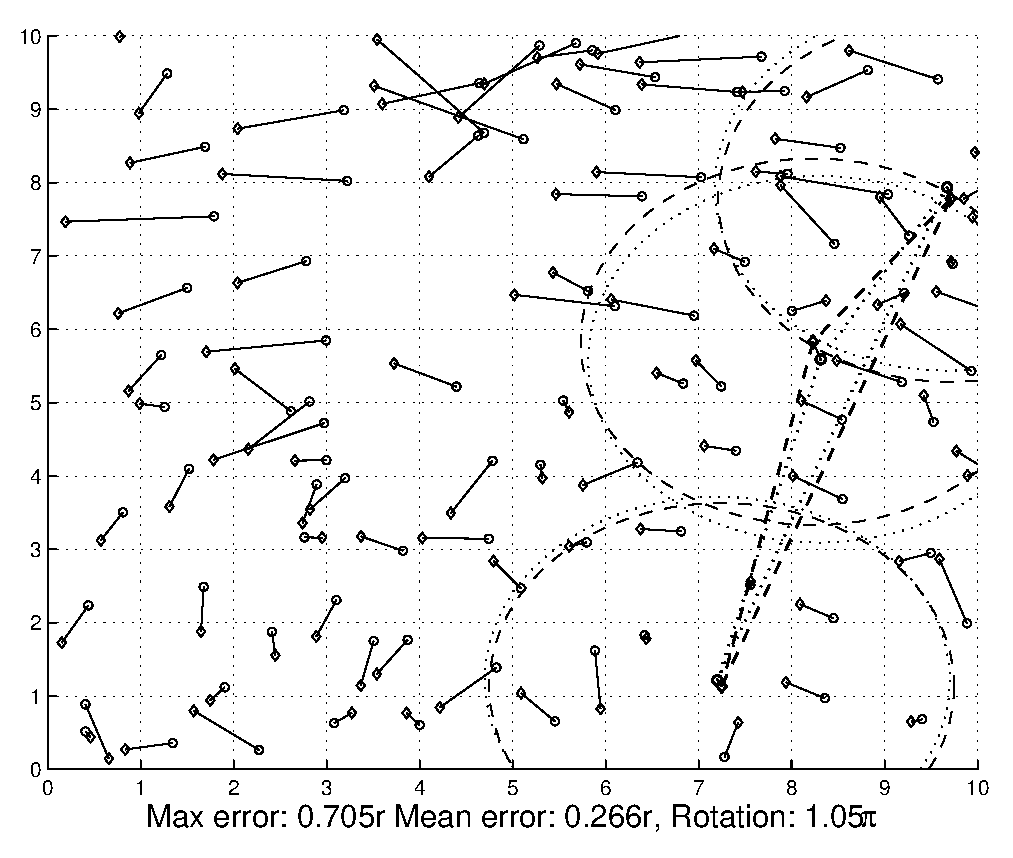
\includegraphics[width=0.5\textwidth]{outliers/AS6/AS6NetworkDiff7.eps}}
	\subfloat[Network A]{\label{fig:AS6NetworkContour7}	
		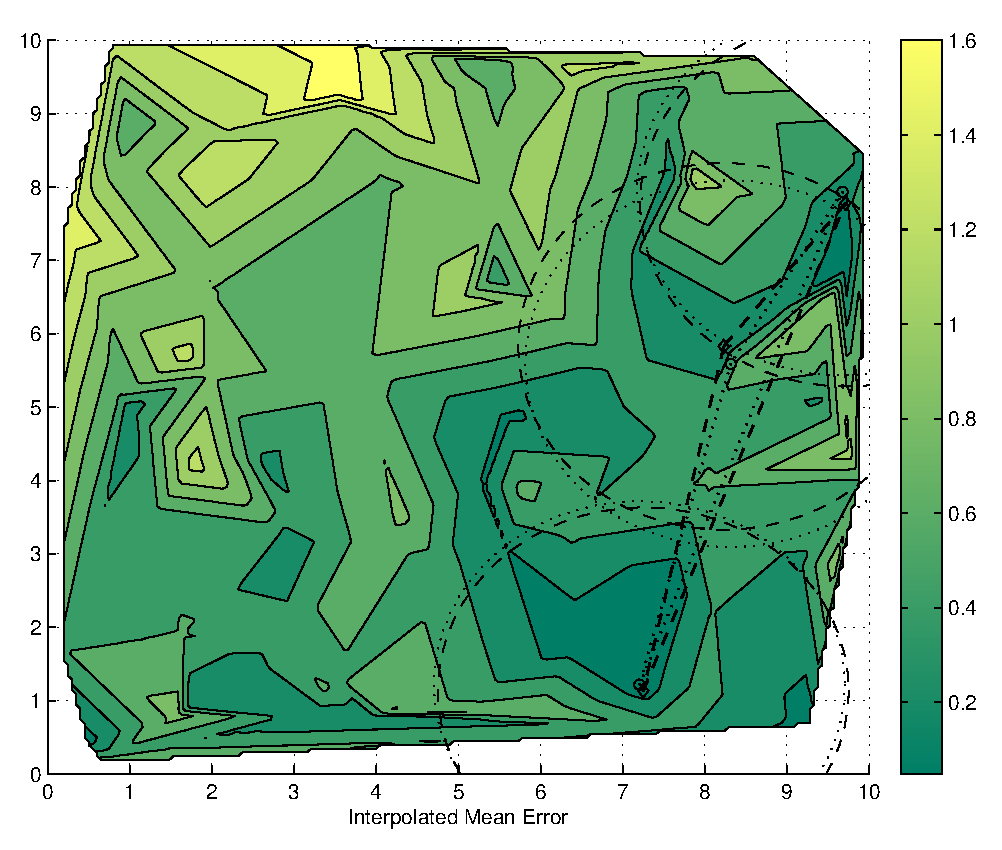
\includegraphics[width=0.5\textwidth]{outliers/AS6/AS6NetworkContour7.eps}}
	\\
	\subfloat[Network B]{\label{fig:AS6NetworkDiff10}
		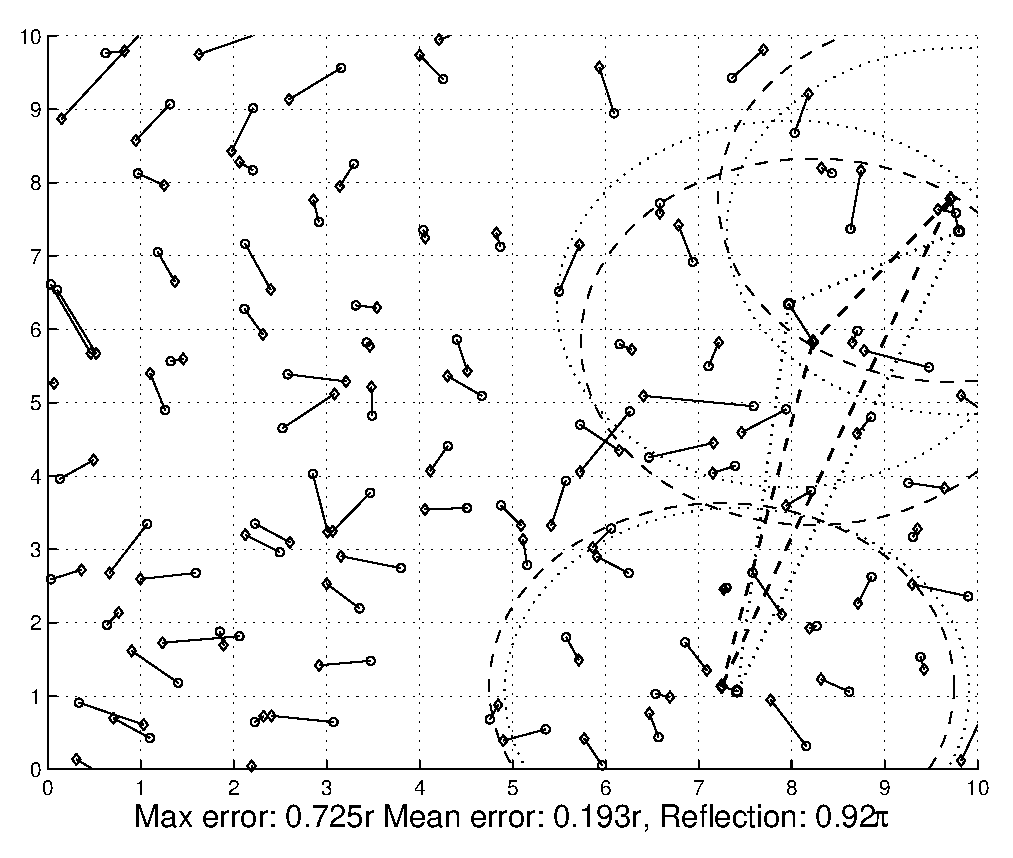
\includegraphics[width=0.5\textwidth]{outliers/AS6/AS6NetworkDiff10.eps}}
	\subfloat[Network B]{\label{fig:AS6NetworkContour10}	
		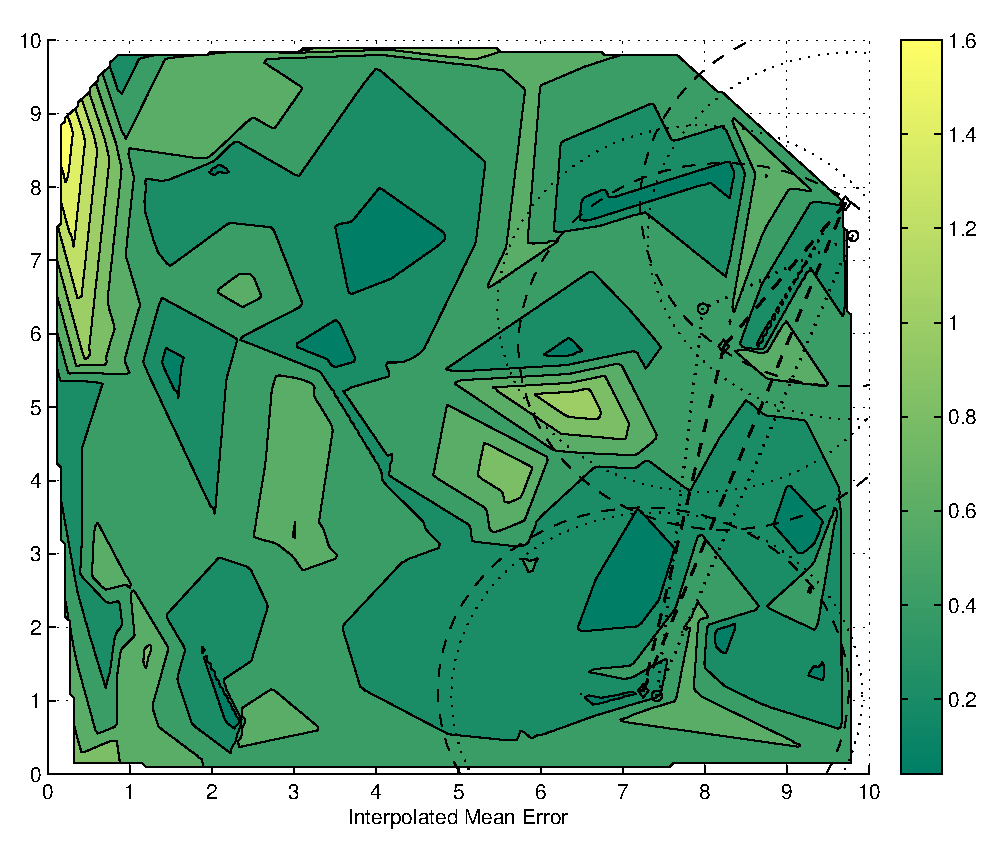
\includegraphics[width=0.5\textwidth]{outliers/AS6/AS6NetworkContour10.eps}}
	\caption{2 different networks with the same anchor set}	
	\label{fig:AS6bad}		
\end{figure}
\begin{figure}
  \centering
	\subfloat[Network C]{\label{fig:AS6NetworkDiff9}
		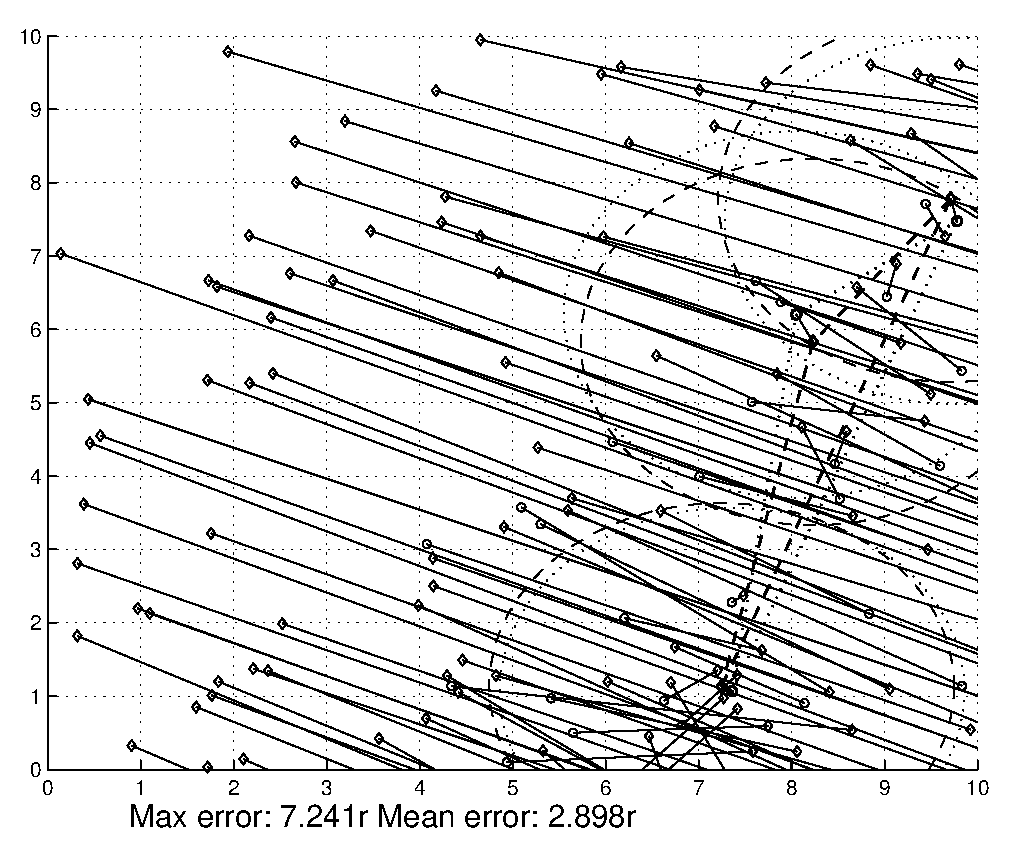
\includegraphics[width=0.5\textwidth]{outliers/AS6/AS6NetworkDiff9.eps}}
	\subfloat[Network C]{\label{fig:AS6NetworkContour9}	
		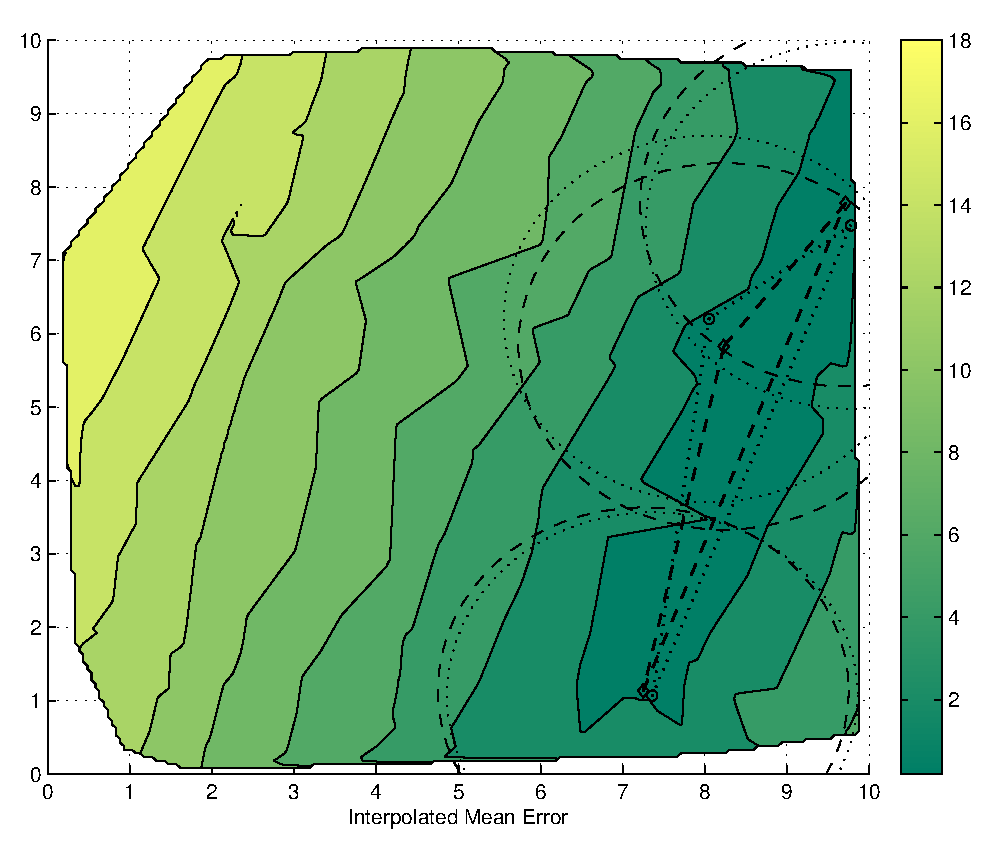
\includegraphics[width=0.5\textwidth]{outliers/AS6/AS6NetworkContour9.eps}}
	\\
	\subfloat[Network D]{\label{AS6NetworkDiff8}
		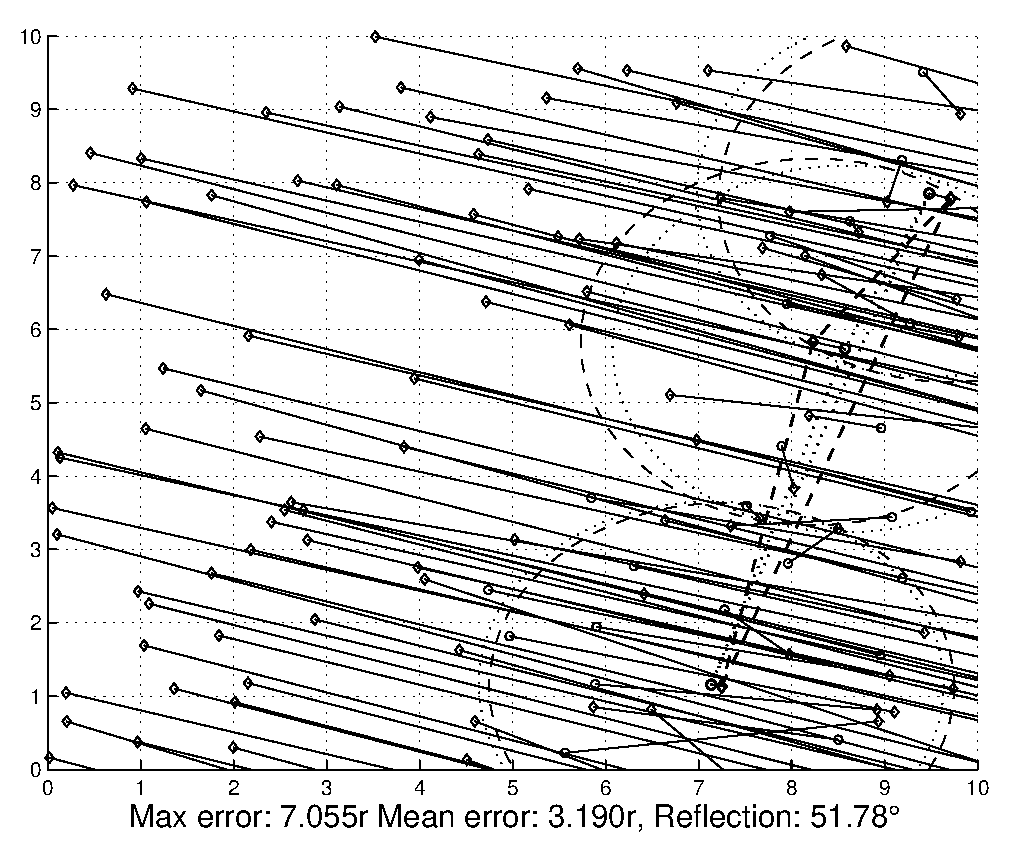
\includegraphics[width=0.5\textwidth]{outliers/AS6/AS6NetworkDiff8.eps}}	
	\subfloat[Network D]{\label{fig:AS6NetworkContour8}	
		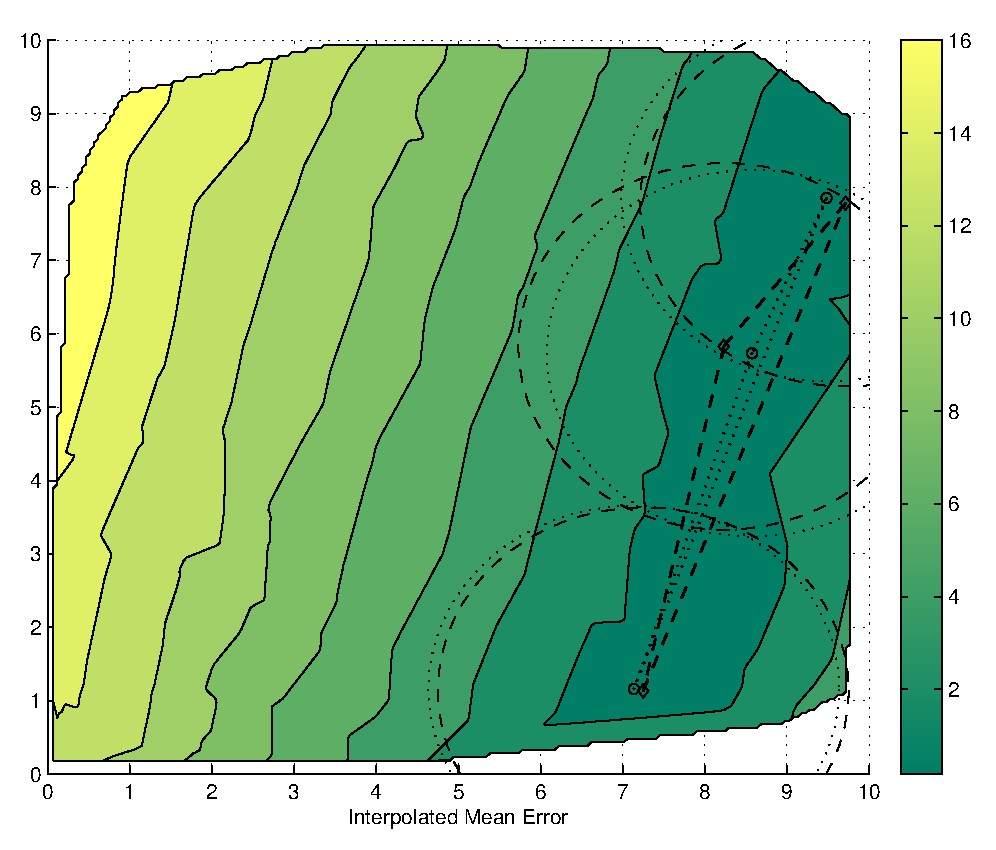
\includegraphics[width=0.5\textwidth]{outliers/AS6/AS6NetworkContour8.eps}}
	\caption{2 more different networks with the same anchor set}	
	\label{fig:AS6bad}
\end{figure}
